\chapter{Экспериментальное исследование и обработка результатов}\label{chapter41}

\section{Постановка эксперимента}

\subsection{Конфигурация экспериментального стенда}

\subsubsection{Аппаратное обеспечение}

Процессоры 2 x Intel Xeon Platinum 8168 CPU @ 2.7 GHz.
Технология Hyper-Threading отключена для уменьшения нежелательного влияния на время обслуживания заявок в системе \cite{LowLatencyHT}.

Оперативная память: DDR4-2666 128 GiB.

\subsubsection{Программное обеспечение}

Операционная система Red Hat Enterprise Linux Server release 7.8 (Maipo).
Ядро Linux 3.10.0-1127.el7.x86\_64

Компилятор C++ Clang 6.0.1.

Стандартная библиотека C++: libstdc++ 8.1.0.

Библиотека Boost.Interprocess 1.68.0.

\subsection{Конфигурация экспериментальной системы}

Система для проведения эксперимента состоит из двух процессов:
\begin{itemize}
\item Процесс-шлюз отвечает за преобразование заявок из формата внешнего мира во внутренний формат системы и обратно. 
\item Процесс-обработчик совершает некоторые преобразования над заявкой и отправляет результат за пределы системы через процесс-шлюз.
\end{itemize}

Процессы выполняются на двух процессорах, расположенных в разных разъемах на материнской плате физического узла.

Снаружи системы находится симулятор внешнего мира. Он генерирует поток заявок в систему и получает результат обработки заявки в системе. Схема взаимодействия процессов в эксперименте представлена на Рисунке \ref{chapter41:SystemSchema}.

\begin{figure}[!h]
\caption{Схема взаимодействия процессов в эксперименте}
\label{chapter41:SystemSchema}
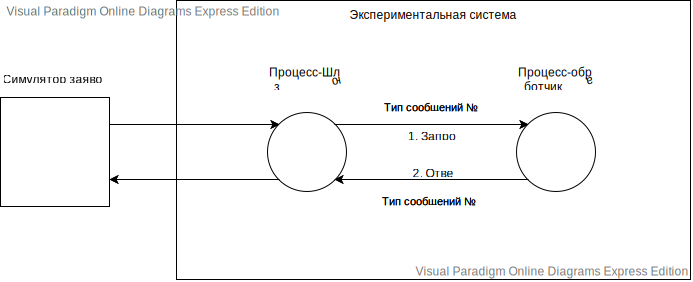
\includegraphics[width=\textwidth]{../../graphics/schemes/SystemSchema}
\end{figure}

В настоящей работе замеряется временная задержка на передачу данных между процессами внутри системы, а именно из процесса-шлюза в процесс-обработчик и обратно (сообщения типа №1 и №2 в запросе и ответе между процессом-шлюзом и процессом обработчиком на Рисунке \ref{chapter41:SystemSchema}).

Процессы системы взаимодействуют используют одно соединение, в рамках которого заявки обрабатываются строго последовательно.
Обслуживание включает в себя: прием заявки, выполнение пользовательской логики над заявкой и, если необходимо, отправка ответа.
Временной задержкой на передачу данных в настоящей работе принимается временной промежуток от начала отправки заявки до \textbf{начала обработки заявки}. Таким образом, возможен случай, когда во время обработки очередной заявки процессом в очереди уже находится следующая заявка, временная задержка на передачу которой, таким образом, увеличится на время обработки текущей заявки.

Данный сценарий актуален для процесса-обработчика, в котором обслуживание заявки осуществляется непосредственно в транспортном потоке \textbf{TBD: Дать определение транспортному потоку}. В случае с процессом-шлюзом транспортный поток только читает и диспетчеризует асинхронную обработку заявки, т.е. не выполняет обработку самой заявки.

\textbf{TBD: надо как- то адекватно это описать}
Пользовательская логика процесс-обработчика в среднем отклоняет 25\% заявок, в то время как 75\% заявок отправляются в процесс-шлюз.

\subsection{Используемые обозначения}
\textbf{TBD: а надо ли оно мне?}

Все величины с, указанные с интервалом, указаны с 95\% доверительной вероятностью.

\begin{itemize}
\item $\Delta$ -- временная задержка между сериями заявок
\item $\delta$ -- временная задержка между заявками в серии
\end{itemize}

\subsection{Характер экспериментальной нагрузки}

Симулятор отправляет в систему заявки сериями с интервалом $\Delta$ в \textit{~10 мс} по \textit{4} заявки в серии с интервалом $\delta$ \textit{~60 мкс} между ними. Так как для каждого эксперимента производился отдельный запуск симулятора, средние значения обозначенных величин приведены для каждого эксперимента отдельно.

\subsection{Время обслуживания заявок в процессах}
\textbf{TBD: разобраться с обработкой соединений и обслуживанием заявок. Должно быть одно слово для обозначения одной сущности.}

На Рисунке \ref{chapter41:EngineLatency} представлена гистограмма времени обслуживания заявок в процессе-обработчике. Время обслуживания заявок с 95\% доверительной вероятностью укладывается в диапазон \textit{13 $\pm$ 7 мкс}.
\begin{figure}[!h]
\caption{Гистограмма времени обслуживания заявки в процессе-обработчике}
\label{chapter41:EngineLatency}
\includegraphics[width=\textwidth]{../../graphics/hist/Engine}
\end{figure}

На Рисунке \ref{chapter41:TRLatency} представлена гистограмма времени обслуживания заявок в процессе-шлюзе. Время обслуживания заявок с 95\% доверительной вероятностью укладывается в диапазон \textit{19 $\pm$ 6 мкс}.
\begin{figure}[!h]
\caption{Гистограмма времени обслуживания заявки в процессе-шлюзе}
\label{chapter41:TRLatency}
\includegraphics[width=\textwidth]{../../graphics/hist/TR}
\end{figure}

\textbf{TBD: а надо ли мне вообще говорить тогда про время обслуживания заявок в процессе-шлюзе? Может, убрать совсем?}
Как было сказано выше, в процессе-шлюзе заявки обслуживания вне транспортного потока, поэтому время обслуживания заявок в процессе-шлюзе не влияет на временную задержку на передачу данных. В случае с процессом-обработчиком значительная часть обслуживания заявки выполняется именно в транспортном потоке, что влияет на временную задержку на передачу данных, т.к. время приема заявки зависит от того, как долго она находилась в очереди.


\section{Результаты экспериментов}

\subsection{Использование TCP для передачи данных}

В качестве точки отсчета в настоящей работе выступает метод межпроцессного взаимодействия на основе TCP, используемый посредством сокетов \textbf{TBD: ссылка на определение и на раздел диссертации} \ref{chapter31:PureTCP}. Гистограмма временной задержки на передачу данных для данного метода приведена на Рисунке \ref{chapter41:FigPureTCP}.

\begin{figure}[!h]
\caption{Гистограмма временной задержки на передачу данных между процессами при использовании TCP}
\label{chapter41:FigPureTCP}
\includegraphics[width=\textwidth]{../../graphics/hist/PureTCP}
\end{figure}

В данном эксперименте симулятор отправляет серию заявок каждые \textit{10 $\pm$ 4 мс} с интервалом \textit{50 $\pm$ 26 мкс}  с коэффициентом доверия 95\%.

В Таблице \ref{chapter41:TablePureTCP} приведены основные временные характеристики данного метода. Временная задержка на передачу данных в обоих направлениях имеет схожие значения.

\begin{table}[!h]
\caption{Основные показатели временной задержки на передачу данных для метода на основе TCP}\label{chapter41:TablePureTCP}
\centering
\begin{tabular}{|l|c|c|}
\hline
\begin{tabular}[c]{@{}l@{}}Направление\\ взаимодействия/\\ Показатель\end{tabular} & \multicolumn{1}{l|}{\begin{tabular}[c]{@{}l@{}}Процесс-шлюз $\rightarrow$\\ Процесс-обработчик\end{tabular}} & \multicolumn{1}{l|}{\begin{tabular}[c]{@{}l@{}}Процесс-обработчик $\rightarrow$\\ Процесс-шлюз\end{tabular}} \\ \hline
min(t), мкс & 9 & 13 \\ \hline
M(t) $\pm$ 95\%, мкс & 27.5 $\pm$ 8.5 & 28 $\pm$ 7 \\ \hline
max(t), мс & 2.1 & 9.2 \\ \hline
\begin{tabular}[c]{@{}l@{}}$\delta$ между\\ сериями, мс\end{tabular} & 10 $\pm$ 4 & 10 $\pm$ 4 \\ \hline
\begin{tabular}[c]{@{}l@{}}$\delta$ между\\ заявками в серии, мкс\end{tabular} & 50 $\pm$ 26 & 87 $\pm$ 32 \\ \hline
\end{tabular}
\end{table}

\subsection{Использование разделяемой памяти для передачи данных}

\subsubsection{Использование TCP для оповещения о появлении данных}

В данном эксперименте симулятор отправляет серию заявок каждые \textit{10 $\pm$ 4 мс} с интервалом \textit{50 $\pm$ 27 мкс} с коэффициентом доверия 95\%.

В данном подразделе приведены данные об экспериментах с методом межпроцессного взаимодействия, описанным в Разделе \ref{chapter31:SignalTCP}.

\begin{figure}[!h]
\caption{Гистограмма временной задержки на передачу данных между процессами при использовании разделяемой памяти для передачи данных и TCP для оповещения о появлении данных в ней}
\label{chapter41:FigSignalTCP}
\includegraphics[width=\textwidth]{../../graphics/hist/SignalTCP}
\end{figure}

В Таблице \ref{chapter41:TableSignalTCP} приведены основные временные характеристики данного метода. Межпроцессное взаимодействие в сторону процесса-обработчика работает быстрее, т.к. в среднем время обслуживания заявок в процессе-обработчике заметно меньше (см. Рисунок \ref{chapter41:EngineLatency}), чем скорость поступления новых заявок, что позволяет использовать оптимизацию, описанную в Разделе \ref{chapter31:SharedMemoryOptimization} \textbf{TBD: сослаться на оптимизацию про отсутствие необходимости отправки новых сигналов, когда старые еще не были обработаны.}.

\begin{table}[!h]
\caption{Основные показатели временной задержки на передачу данных для метода, использующего разделяемую памяти для передачи данных и TCP для оповещения о появлении данных в ней}\label{chapter41:TableSignalTCP}
\centering
\begin{tabular}{|l|c|c|}
\hline
\begin{tabular}[c]{@{}l@{}}Направление\\ взаимодействия/\\ Показатель\end{tabular} & \multicolumn{1}{l|}{\begin{tabular}[c]{@{}l@{}}Процесс-шлюз $\rightarrow$\\ Процесс-обработчик\end{tabular}} & \multicolumn{1}{l|}{\begin{tabular}[c]{@{}l@{}}Процесс-обработчик $\rightarrow$\\ Процесс-шлюз\end{tabular}} \\ \hline
min(t), мкс & 1 & 3 \\ \hline
M(t) $\pm$ 95\%, мкс & 22.5 $\pm$ 12.5 & 27.5 $\pm$ 5.5 \\ \hline
max(t), мс & 3 & 9ю8 \\ \hline
\begin{tabular}[c]{@{}l@{}}$\delta$ между\\ сериями, мс\end{tabular} & 10 $\pm$ 4 & 10 $\pm$ 4 \\ \hline
\begin{tabular}[c]{@{}l@{}}$\delta$ между\\ заявками в серии, мкс\end{tabular} & 50 $\pm$ 27 & 87 $\pm$ 32 \\ \hline
\end{tabular}
\end{table}

\subsubsection{Использование мультиплексора в разделяемой памяти для оповещения о появлении данных}

В данном подразделе приведены данные об экспериментах с методом межпроцессного взаимодействия, описанным в Разделе \ref{chapter31:SignalTCP}.

\paragraph{Блокирующие методы}

В блокирующих методах поток мультиплексора событий использует примитив \textit{futex} \textbf{Может, сослаться на определение futex?} для пассивного ожидания новых сигналов (см. Раздел \ref{chapter31:BlockingMux}).

\subparagraph{Диспетчеризация и обработка соединений по модели "Полусинхронный/Полуреактивный"}

В данном эксперименте симулятор отправляет серию заявок каждые \textit{10 $\pm$ 4 мс} с интервалом \textit{51 $\pm$ 28 мкс} с коэффициентом доверия 95\%.

В данном подразделе приведены данные об экспериментах с методом межпроцессного взаимодействия, описанным в Разделе \ref{chapter31:BlockingHSHA}.

В Таблице \ref{chapter41:TableBlockingHSHA} приведены основные временные характеристики данного метода. \textbf{TBD}

На Рисунке \ref{chapter41:FigBlockingHSHA} приведена плотность вероятности временной задержки на передачу данных для данного метода.

\begin{figure}[!h]
\caption{Гистограмма временной задержки на передачу данных между процессами для метода, использующего разделяемую память для передачи данных, блокирующий мультиплексор в разделяемой памяти и модель ''Полусинхронный/Полуреактивный`` при обслуживании заявок}
\label{chapter41:FigBlockingHSHA}
\includegraphics[width=\textwidth]{../../graphics/hist/BlockingHSHA}
\end{figure}
%
%В Таблице \ref{chapter41:TableBlockingHSHA} приведены основные временные характеристики данного метода. Межпроцессное взаимодействие в сторону процесса-обработчика работает быстрее, т.к. в среднем время обслуживания заявок в процессе-обработчике заметно меньше (см. Рисунок \ref{chapter41:EngineLatency}), чем скорость поступления новых заявок, что позволяет использовать оптимизацию, описанную в Разделе \ref{chapter31:SharedMemoryOptimization} \textbf{TBD: сослаться на оптимизацию про отсутствие необходимости отправки новых сигналов, когда старые еще не были обработаны.}.

\begin{table}[!h]
\caption{Основные показатели временной задержки на передачу данных между процессами для метода, использующего разделяемую память для передачи данных, блокирующий мультиплексор в разделяемой памяти и модель ''Полусинхронный/Полуреактивный`` при обслуживании заявок}\label{chapter41:TableBlockingHSHA}
\centering
\begin{tabular}{|l|c|c|}
\hline
\begin{tabular}[c]{@{}l@{}}Направление\\ взаимодействия/\\ Показатель\end{tabular} & \multicolumn{1}{l|}{\begin{tabular}[c]{@{}l@{}}Процесс-шлюз $\rightarrow$\\ Процесс-обработчик\end{tabular}} & \multicolumn{1}{l|}{\begin{tabular}[c]{@{}l@{}}Процесс-обработчик $\rightarrow$\\ Процесс-шлюз\end{tabular}} \\ \hline
min(t), мкс & 1 & 3 \\ \hline
M(t) $\pm$ 95\%, мкс & 12.5 $\pm$ 5.5 & 11.5 $\pm$ 2.5 \\ \hline
max(t), мс & 6.9 & 11.6 \\ \hline
\begin{tabular}[c]{@{}l@{}}$\delta$ между\\ сериями, мс\end{tabular} & 10 $\pm$ 4 & 10 $\pm$ 4 \\ \hline
\begin{tabular}[c]{@{}l@{}}$\delta$ между\\ заявками в серии, мкс\end{tabular} & 51 $\pm$ 28 & 91 $\pm$ 36 \\ \hline
\end{tabular}
\end{table}

\subparagraph{Диспетчеризация и обработка соединений по модели "Лидер/Последователи"}

В данном эксперименте симулятор отправляет серию заявок каждые \textit{8.4 $\pm$ 5.3 мс} с интервалом \textit{52 $\pm$ 28 мкс} с коэффициентом доверия 95\%.

В данном подразделе приведены данные об экспериментах с методом межпроцессного взаимодействия, описанным в Разделе \ref{chapter31:BlockingLF}.

В Таблице \ref{chapter41:TableBlockingLF} приведены основные временные характеристики данного метода. \textbf{TBD}

На Рисунке \ref{chapter41:FigBlockingLF} приведена плотность вероятности временной задержки на передачу данных для данного метода.

\begin{figure}[!h]
\caption{Гистограмма временной задержки на передачу данных между процессами для метода, использующего разделяемую память для передачи данных, блокирующий мультиплексор в разделяемой памяти и модель ''Лидер/Последователи`` при обслуживании заявок}
\label{chapter41:FigBlockingLF}
\includegraphics[width=\textwidth]{../../graphics/hist/BlockingLF}
\end{figure}
%
%В Таблице \ref{chapter41:TableBlockingHSHA} приведены основные временные характеристики данного метода. Межпроцессное взаимодействие в сторону процесса-обработчика работает быстрее, т.к. в среднем время обслуживания заявок в процессе-обработчике заметно меньше (см. Рисунок \ref{chapter41:EngineLatency}), чем скорость поступления новых заявок, что позволяет использовать оптимизацию, описанную в Разделе \ref{chapter31:SharedMemoryOptimization} \textbf{TBD: сослаться на оптимизацию про отсутствие необходимости отправки новых сигналов, когда старые еще не были обработаны.}.

\begin{table}[!h]
\caption{Основные показатели временной задержки на передачу данных между процессами для метода, использующего разделяемую память для передачи данных, блокирующий мультиплексор в разделяемой памяти и модель ''Лидер/Последователи`` при обслуживании заявок}\label{chapter41:TableBlockingLF}
\centering
\begin{tabular}{|l|c|c|}
\hline
\begin{tabular}[c]{@{}l@{}}Направление\\ взаимодействия/\\ Показатель\end{tabular} & \multicolumn{1}{l|}{\begin{tabular}[c]{@{}l@{}}Процесс-шлюз $\rightarrow$\\ Процесс-обработчик\end{tabular}} & \multicolumn{1}{l|}{\begin{tabular}[c]{@{}l@{}}Процесс-обработчик $\rightarrow$\\ Процесс-шлюз\end{tabular}} \\ \hline
min(t), мкс & 1 & 2 \\ \hline
M(t) $\pm$ 95\%, мкс & 11.5 $\pm$ 6.5 & 9.5 $\pm$ 1.5 \\ \hline
max(t), мс & 2.4 & 9.5 \\ \hline
\begin{tabular}[c]{@{}l@{}}$\delta$ между\\ сериями, мс\end{tabular} & 8.4 $\pm$ 5.3 & 8.4 $\pm$ 5.3 \\ \hline
\begin{tabular}[c]{@{}l@{}}$\delta$ между\\ заявками в серии, мкс\end{tabular} & 52 $\pm$ 29 & 90 $\pm$ 35 \\ \hline
\end{tabular}
\end{table}





\paragraph{Неблокирующий метод}

В неблокирующем методе поток мультиплексора событий метод активного ожидания новых сигналов (см. Раздел \ref{chapter31:NonBlockingMux}). В данном параграфе рассматривается исключительно модель обслуживания заявок ''Лидер/Последователи`` т.к. в параграфе выше она показала лучшие результаты по сравнению с моделью ''Полусинхронный/Полуреактивный``.

\subparagraph{Диспетчеризация и обработка соединений по модели "Лидер/Последователи"}

В данном эксперименте симулятор отправляет серию заявок каждые \textit{7.4 $\pm$ 5.9 мс} с интервалом \textit{55 $\pm$ 32 мкс} с коэффициентом доверия 95\%.

В данном подразделе приведены данные об экспериментах с методом межпроцессного взаимодействия, описанным в Разделе \ref{chapter31:NonBlockingLF}.

В Таблице \ref{chapter41:TableNonBlockingLF} приведены основные временные характеристики данного метода. \textbf{TBD}

На Рисунке \ref{chapter41:FigNonBlockingLF} приведена плотность вероятности временной задержки на передачу данных для данного метода.

\begin{figure}[!h]
\caption{Гистограмма временной задержки на передачу данных между процессами для метода, использующего разделяемую память для передачи данных, блокирующий мультиплексор в разделяемой памяти и модель ''Лидер/Последователи`` при обслуживании заявок}
\label{chapter41:FigNonBlockingLF}
\includegraphics[width=\textwidth]{../../graphics/hist/NonBlockingLF}
\end{figure}
%
%В Таблице \ref{chapter41:TableBlockingHSHA} приведены основные временные характеристики данного метода. Межпроцессное взаимодействие в сторону процесса-обработчика работает быстрее, т.к. в среднем время обслуживания заявок в процессе-обработчике заметно меньше (см. Рисунок \ref{chapter41:EngineLatency}), чем скорость поступления новых заявок, что позволяет использовать оптимизацию, описанную в Разделе \ref{chapter31:SharedMemoryOptimization} \textbf{TBD: сослаться на оптимизацию про отсутствие необходимости отправки новых сигналов, когда старые еще не были обработаны.}.

\begin{table}[!h]
\caption{Основные показатели временной задержки на передачу данных между процессами для метода, использующего разделяемую память для передачи данных, блокирующий мультиплексор в разделяемой памяти и модель ''Лидер/Последователи`` при обслуживании заявок}\label{chapter41:TableNonBlockingLF}
\centering
\begin{tabular}{|l|c|c|}
\hline
\begin{tabular}[c]{@{}l@{}}Направление\\ взаимодействия/\\ Показатель\end{tabular} & \multicolumn{1}{l|}{\begin{tabular}[c]{@{}l@{}}Процесс-шлюз $\rightarrow$\\ Процесс-обработчик\end{tabular}} & \multicolumn{1}{l|}{\begin{tabular}[c]{@{}l@{}}Процесс-обработчик $\rightarrow$\\ Процесс-шлюз\end{tabular}} \\ \hline
min(t), мкс & 1 & 3 \\ \hline
M(t) $\pm$ 95\%, мкс & 7 $\pm$ 4 & 5 $\pm$ 1 \\ \hline
max(t), мс & 8.5 & 0.003 \\ \hline
\begin{tabular}[c]{@{}l@{}}$\delta$ между\\ сериями, мс\end{tabular} & 7.4 $\pm$ 5.9 & 7.4 $\pm$ 5.9 \\ \hline
\begin{tabular}[c]{@{}l@{}}$\delta$ между\\ заявками в серии, мкс\end{tabular} & 58 $\pm$ 35 & 167 $\pm$ 113 \\ \hline
\end{tabular}
\end{table}

\chapterconclusion

Проведено экспериментальное сравнение разработанных методов межпроцессного взаимодействия.
\begin{enumerate}
\item Методы межпроцессного взаимодействия, использующие мультиплексор в разделяемой памяти для оповещения о появлении данных в очереди в разделяемой памяти имеют существенно меньшую временную задержку на передачу данных, чем метод, использующий для этого TCP. А именно, $11.5 \pm 6.5 \text{ мкс и } 9.5 \pm 1.5 \text{ мкс}$ для пассивного варианта ''Лидер/Последователи`` против $22.5 \pm 12.5 \text{ мкс и } 27.5 \pm 5.5 \text{ мкс}$ для TCP с передачей данных через очередь в разделяемой памяти.
\item В семействе пассивных методов межпроцессного взаимодействия на основе мультиплексора в разделяемой памяти наименьшую временную задержку на передачу данных показала вариация с использованием метода обслуживания заявок ''Лидер/Последователи``, а именно $11.5 \pm 6.5 \text{ мкс и } 9.5 \pm 1.5 \text{ мкс}$ против $12.5 \pm 5.5 \text{ мкс и } 11.5 \pm 2.5 \text{ мкс}$.
\item Самой низкой временной задержки на передачу данных удалось добиться при использовании активно опрашивающей мультиплексор вариации метода межпроцессного взаимодействия, использующего метод ''Лидер/Последователи`` при обслуживании заявок. А именно, $6 \pm 2 \text{ мкс и } 5 \pm 1 \text{ мкс}$.
\item При использовании пассивных методов на основе мультиплексора в разделяемой памяти заметны эффекты от обслуживания заявок в транспортном потоке на временную задержку на передачу данных. В проведенном эксперименте в процессе-шлюзе заявки частично обслуживаются именно в транспортном потоке, из-за чего могут образовываться очереди и увеличиваться временная задержка на передачу данных. В активно опрашивающем методе этот эффект не заметен, так как временная задержка на передачу данных меньше, соответственно, меньше временная задержка реакции на очередную заявку и, следовательно, меньше возможностей для формирования очереди из заявок.
\item Активно опрашивающий мультиплексор метод обладает существенным недостатком. поток, активно опрашивающий мультиплексор в разделяемой памяти, может быть вытеснен с процессора по окончании отведенного ему кванта процессорного времени -- 100 миллисекунд. В проведенном эксперименте данный эффект не наблюдается, так как серии заявок отправляются симулятором в систему на порядок чаще, каждые $10 \pm 4 \text{ миллисекунд}$. Данный недостаток может быть необходимо разрешить для обеспечения должного уровня качества обслуживания заявок в системе.
\end{enumerate}